\chapter{The Internet Of Things}
\label{sec:IoT}
The Internet of Things (IoT) is a paradigm to which we put more and more attention in the scientific community\cite{atzori2010iotsurvey}.
\todo{It comes as a necessity}, since new services must be provided to cope the new era of \textit{\textbf{"Smart Things"}}, which leverages existing networking infrastructure and communication technologies.
Such \textit{smart} capabilities of future facilities will bring a radical change in human relationships with his everyday environment.

Moreover, most of the efforts to create this new services for people should focus in the seamless integration of new technologies, following the vision of ubiquitous computing proposed by Mark Weiser\cite{weiser1999ubiquitous}.
Even though when humans might interact with this IoT infrastructure, their activity should be limited to the activation/deactivation of services, as well as a very small amount of configurations.

Pieces of the IoT are already present in everyday's life, such as sensor networks in smart cities, personal smartphones, RFID tags in many retail stores, and so on.
However, the seamless integration of this pieces still have several issues, from the development and deployment of services, to the usability.

Likewise, a huge variety of connected objects are now available in the market for a specific use, most of them known as \textit{"wearables"}.
While its usability is quite friendly, the interaction with other devices is very limited.
Usually it communicates with the user through a smart phone, and in some cases they embed a user interface (UI), i.e. a display in the case of smart watches.

Into this category we can also include other objects called "smart sensors", like plant monitors\cite{bolliger2007koubachi}, which are able to give environmental measurements through Bluetooth Low Energy(BLE) notifications, or web based notifications for a more sophisticated sensor\footnote{http://www.koubachi.com/products/pro/}.

This devices are also part of the IoT\cite{wei2014wearables}, however, most of the technologies used to create them are proprietary, which complicates interoperability with other similar devices.
In addition, most of the services provided by this objects are merely extensions of a bigger device, making them a subset of the IoT.
For instance, a smart watch will provide notifications and small messages that the smart phone is already able to manage, with the advantage that we can put attention more quickly, contrasting the vision of ubiquitous computing stated above.
However, one main benefit of this is that the wave radiation emitted by a wearable is, by far, less important than the phone's, allowing a distancing from the phone radio emissions.

Another important area of research for the IoT is in the industrial field\cite{lidaxu2014iiotsurvey}.
Applications in this area are emerging along with the robustness that new network infrastructures provide, since most of the usages require real-time responsiveness.
Industries can leverage the IoT to increase performance and reduce waste of resources.
While sensor networks are already present in all industrial scenarios, they are intended exclusively for automation and productivity.
Resource availability, production tracking and non-supervisory process monitoring can be improved by an ad-hoc data analysis, which industrial IoT (IIoT) can provide.
This new infrastructure can be deployed to obtain data about resources usage, such as electricity, water, gas, and so on.
It exists big data based solutions\todo{\cite{}Erwan energiency} which could leverage all the generated data, in order to find energy leaks, which can bring considerable savings. 


%Some organizations, like the IEEE\footnote{IEEE, towards an IoT definition http://goo.gl/u4AjEd}, are proposing a complete definition to the IoT, but it is hard to have a common consensus.
%However, for this thesis I will propose a definition from my experience and my own understanding, also based in those definitions.

\section{The IoT at a glance}
Nowadays, the current Internet, or the Internet of people, is driven by a set of technologies which were developed, extended and improved for the sake of human beings.
This \textit{\textbf{classical}} Internet technologies are those which are used, for instance, in computers, tablets, smart-phones, smart TVs and streaming boxes, just to name a few.
Users reach this Internet in form of web pages, audio and video streaming, mobile applications, and so on.
In the literature, these are called \textit{\textbf{web services}}, which are provided from other machines known as \textit{\textbf{web servers}}.
Web technologies are very well standardized, which allows a direct use of this information for any device implementing such standards.

On the other hand, systems that does not provide direct communication to the user, but on the contrary, communicate exclusively with other machines, should use different means to reach the Internet.
For this, a new infrastructure that provides connectivity to devices of this kind is then necessary, and must leverage, as much as possible, existing frameworks to ease their integration and exploitation.
That's why the Internet of Things should make use of different approaches, since the nature of their data and provided services differ  significantly from classical web services.
The \textit{\textbf{web of things}}\cite{duquennoy2009webofthings} is the goal to achieve for this new infrastructure.

\section{Towards an infrastructure for IoT}
\label{sec:IoTInfra}
%Smart city -> system of systems
An IoT infrastructure can be defined as a set of interconnected objects that leverage one or more Internet protocols (IP), in order to exchange information about the tasks for which they were programmed.

This infrastructure must be able to support connectivity and interoperability for a huge number of devices of all nature, from a very small sensor to the cloud.
Furthermore, compatibility with the current Internet basis should be mandatory, in order to take advantage of its robustness.

Existing deployments similar to the described above, such as smart cities, can be an example of large scale systems that could represent an IoT infrastructure.
Indeed, the services provided by smart cities can be compared in scale and complexity to those that the IoT aims to bring.
Such features make its deployment very challenging, since the heterogeneity of the participants complicate the development of standard communication protocols and cross-platform applications.

\begin{figure}[htb]
	\centering
	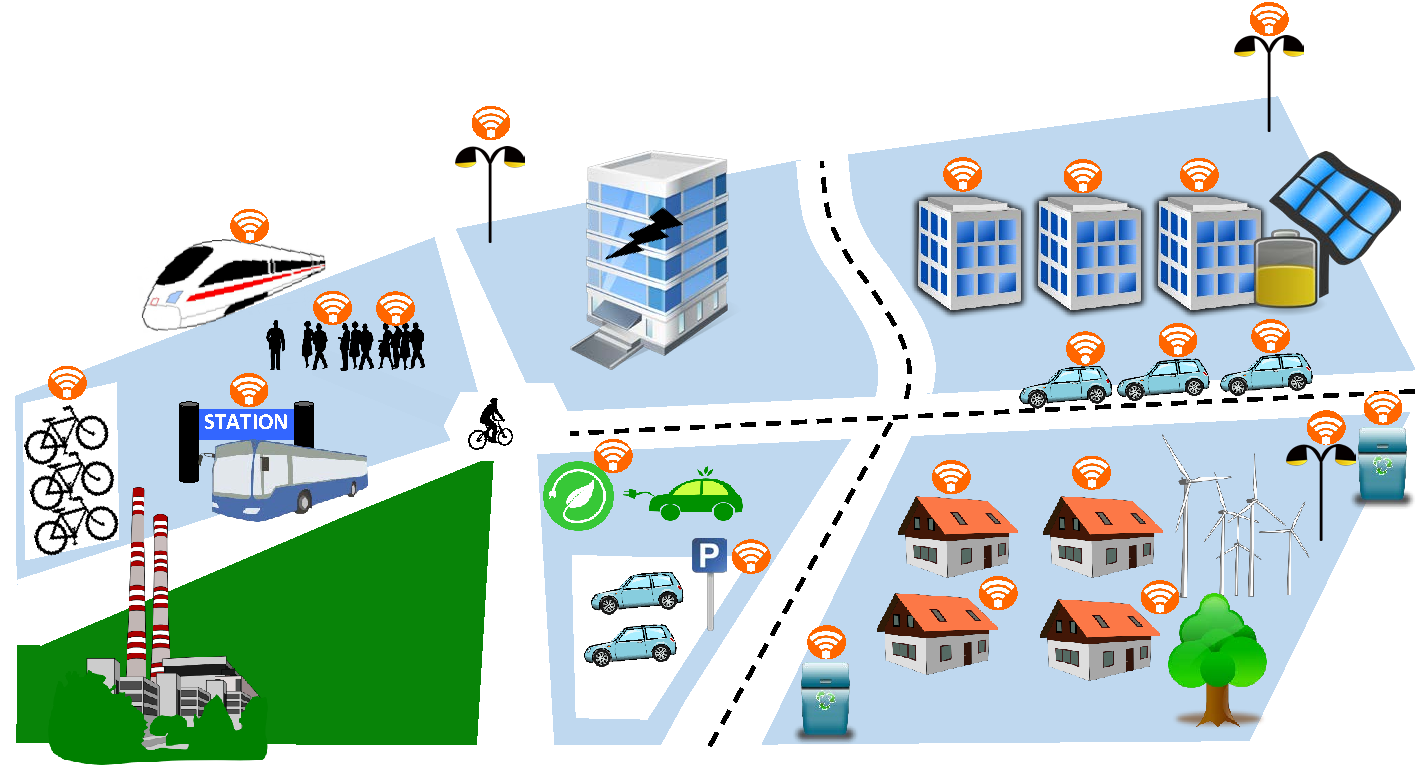
\includegraphics[width=1\columnwidth]{chapters/background.images/SmartCity_comm.pdf}
	\caption{A Smart City deployment}
	\label{fig:SmartCity}
\end{figure}

In a smart city deployment\cite{smartsantander}, users can benefit from the services derived from different interactions performed between each participant.
In figure \ref{fig:SmartCity} we can observe the diverse participants and its very particular nature, which comes from small embedded environmental sensors to connected cars and smart grids.
A smart city envelops a wide range of devices that differs, mainly, in its communication capabilities.
For instance, networks already deployed in smart buildings make use of particular technologies, as known as "building automation" (BA) protocols.
In contrast, environmental sensors deployed in the city to measure pollution and air quality, utilize protocols typical of Wireless Sensor Networks (WSN)\cite{Akyildiz2002WSN}.
However, such deployments have many points in common.
Both are of a very distributed nature, which means that services provided come from the combination of all data produced by each device, and finally available for exploitation as a whole.
In addition, devices being part of this networks have comparable hardware capabilities, which allows a similar application development environment.

In a typical use case, an user who inhabits a smart building can know if his electric car is fully charged and ready to go, while checking in his smart phone the traffic conditions from there to his office.
At the same time, the smart building could use the electric car as a storage of the building's produced energy, and publish its performance.
Moreover, this system is able to propose other options for transportation, since it is connected to the public mobility network, which provides real time information about buses, public bike availability, and so on.
In addition, the user can also know which are the conditions of air quality and temperature, using the smart city's weather service.
All this \textit{\textbf{"connected world"}} will bring lots of improvements to life quality, as well as a better performance of energy consumption and production, which is a major concern.

In the French Building Automation domain, organizations like the Smart Building Alliance\footnote{http://www.smartbuildingsalliance.org/} are engaged to ease the development of this kind of smart environments, in order to respond to the challenges \textbf{raised by the climate change, pollution and better quality of life demand in modern cities.}

In this very particular scenario of smart buildings, several needed features could be pointed out:

\begin{enumerate}
	\item Interoperability between local equipment
	\item Web services APIs
	\item Data access
	\item Privacy and security
\end{enumerate}

Thus far, this requirements can be met by present building automation technologies.
However, the current issue consist in upgrade existing buildings to this new claims.
This is very challenging, since classical solutions for BA are developed in a statical fashion, i.e. allowing the control and supervision of services like heating, ventilation, and air conditioning (HVAC), without taking into account the future evolutions that buildings can perform.
Furthermore, the very complex deployment of this systems make its adoption very costly, since configuration and further changes must be made by experts.

Let's take the example of an old building that are being refurbished to meet the new energy consumption requirements.
First of all, the building must be analyzed.
A sensor deployment is necessary to find its current performance and the parts that need urgent attention, like structural damages or thermal leaks.
Once the information is gathered and the possible reparations are done, a second step is to replace all the previous sensors for new ones, which will perform the supervision and control of the new added features.
This could be avoid if the first deployment offer adaptive characteristics, reducing costs and time.

In a similar way, a new building which already have sensors an actuators, can change its use and consequently its behavior.
For instance, let's imagine a complete floor full of offices that changes its occupants, from a logistics enterprise to a government agency.
A complete change in the policies for the services provided by the building will be needed, forcing the deployment of new configurations for all sensors and actuators that could be present in the floor, such as new access controls, lighting and HVAC requirements and parking assignment, just to name a few.
Again, an adaptive approach could facilitate this tasks.

Solutions that come from the Information and Communication Technologies (ICT) field should be studied, in order to find a new way to develop, deploy and maintain this infrastructure.
In particular, the research done in Software Engineering (SE) could be useful to explore the issues mentioned above, since solutions for distributed systems, which are very close to the IoT environment, have been studied since long time ago by this branch.
For instance, Meta-Modeling frameworks are already used to perform smart grid data analysis\cite{hartmann2014realisticsmartgrid}, which seems to be very convenient and efficient.



\todo{Make the link}
-----------------------------------------------------------------------------------

\section{A Building Automation scenario}
\label{sec:BAScenario}
As depicted in figure \ref{fig:SmartCity}, the heterogeneity between actors in a smart city requires software development for different platforms.
Indeed, development environments can differ drastically from an scenario to another.

\begin{figure}[htb]
	\centering
	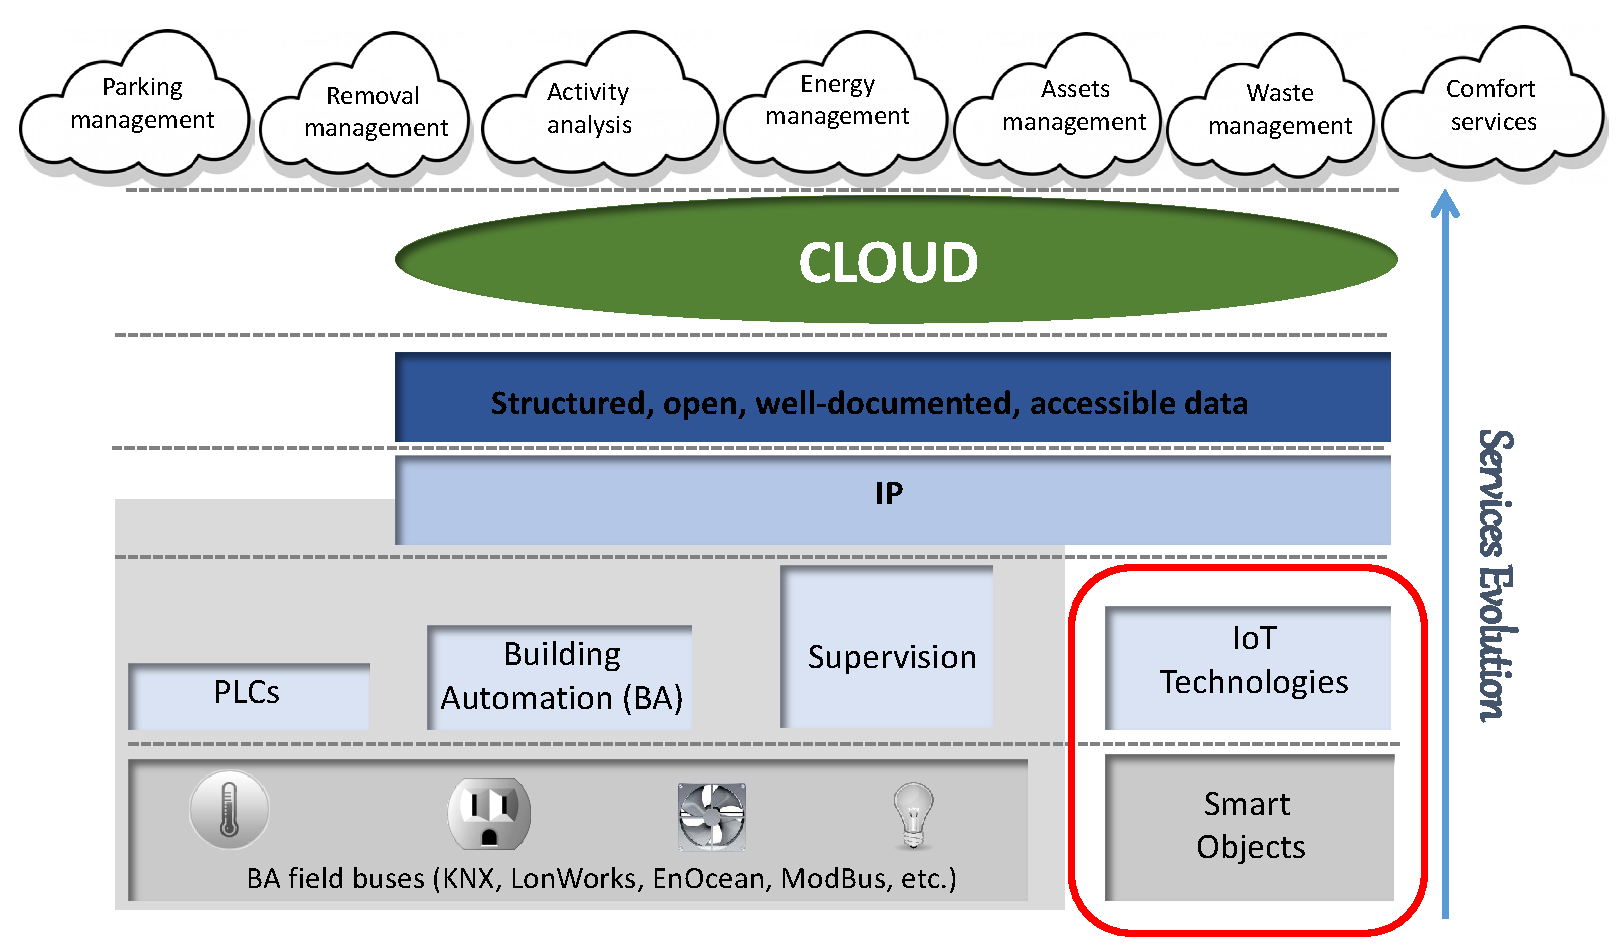
\includegraphics[width=1\columnwidth]{chapters/background.images/SmartServices.pdf}
	\caption{Smart Building environment}
	\label{fig:SmartServices}
\end{figure}

In the case of the smart building environment, we can found several technologies that require many skills and players, since complexity is divided in different levels.

In a bottom-up manner, as shown in figure \ref{fig:SmartServices}, we found in the first place the common sensors present in a building, such as temperature, humidity, luminosity, gas, and so on. 
It also includes all meters like electricity, water and gas, which are the common services available in a building.
In addition, this layer contains all the necessary actuators to control this services, the most common being valves for heating, dampers for ventilation, lights, blinds, and so on.
Most of this devices are built using microcontrollers (MCU) (\todo{should I explain what a MCU is?}), since they are the cheapest and easiest way to perform small measurements, as well as implement one or more communication protocols.

Afterwards, there is an automation layer, which obtains the instantaneous data coming from sensors and meters that, following the programmed algorithms in a Programmable Logic Controller (PLC), execute actions i.e. open/close a valve or turn on/off lights.

A supervision layer then store all the generated data locally, to provide visualizations of the state of the building, either present or past.
Supervisors are often deployed in industrial PCs, servers, or other high-end computer.
This is required due to the very complex data processing needed to represent all the functional features present in the building, as well as a very rich dynamic visual imagery offered to the user.

At this point, this infrastructure is able to communicate using IP protocols, implemented at the automation layer.
Most of BA PLCs provide IP implementations out of the box, either as a gateway (KNX/IP, LonWorks/IP, BACNet/IP, etc.)\cite{kastner2005commbas} or using proprietary modules available from the constructors.
Thanks to this, the upper layers can access, in a \textit{"web fashion"} (i.e. using OPC, oBIX, etc.)\cite{neugschwandtner2007knxtoobix}, to all this data in order to perform cloud-based manipulations.
Research done in this area has interesting results\cite{jung2013bainsmartcities}, but the approaches are often based in gateway developments, which implies an additional software and hardware layer.
This also complicates the evolution of this services, since the required data provided by the lower layers depends on the configurations and embedded software provided from the first deployment.
As explained in section \ref{sec:IoTInfra}, reconfiguration and deployment of new software at low level is a very challenging task.
Thus, a more transparent way to provide web services from the lower layers could be the most efficient approach.
Moreover, allowing a direct communication to this layer would enable access to the configurations and software already installed, offering a remote way to make modifications.
However, current BA devices make use of field buses which are often proprietary, thus adaptability at the firmware level is almost impossible.
While reconfigurations are possible, the very complex protocols make this task very difficult, much more when equipment from different constructors is present.

Thus far, current BA deployments seem to be very difficult to adapt and reconfigure, therefore a new deployment should be proposed.
Since the most viable way to allow evolution of services resides in the adaptation capabilities of the lower layer discussed above, the research efforts will be conducted to this particular case.
The red circle shown in figure \ref{fig:SmartServices} enclose the proposed alternative to the BA approach, which will be explained in the next section.

--------------------------------------------------------------------------------------------\\
\todo{Make the link with this, it should be easier since the scope is now the smart building scenario}


\section{Focusing on constrained devices}
As explained in the previous section, the lower layer of the proposed IoT infrastructure is composed of devices which have low cost, flexible placement and rapid software development as their main features.
Since the goal is to enhance this devices with web features, a new layer must be proposed to replace the existing one, in which web services could be deployed.
However, due to the constrained computational resources of this objects, \textbf{classical} implementations of Internet protocols cannot run in this constrained environment.
I highlight \textit{classical} because interoperability between objects is easier to achieve using the Internet infrastructure that already exists.

The available resources will depend in the function that the object was intended to achieve, and will also be driven by a specific placement and connectivity.
The usage of this objects can be very varied, from common sensing/actuating tasks (temperature, humidity, air quality, HVAC, access control) to small algorithms that provide basic functionalities, such as thermostats, coffee machines, traffic monitors, and so on.
For instance, objects used for environmental sensing applications often need to be installed at a specific place\cite{younis2008placement}, which can be hard to reach. 
This forces to either reach the sensors with a specific cable, for both power and network connectivity, or use wireless communications.
On the other hand, for other devices like home appliances or smart meters, the placement is often already defined, and they can be easily connected to an existing network.

For the first kind of applications mentioned above, wireless communications seem to be very convenient, while in the second example, a wired connection can already exist or could be easy to provide.
The communication method can determine the way we power the device, either using batteries or the electricity network.
Thus, two kind of objects with different hardware capabilities can be present in this IoT infrastructure, which we can separate into:

\begin{itemize}
	\item Constrained devices. These are battery powered wireless devices which have no more than 1MB of RAM and 2MB of ROM (program data), offering a very efficient energy management. The mono-core CPU clock runs at less than a hundred megahertz.
	\item Non-constrained devices. Wall-powered System on a Chip (SoC) devices counting with several megabytes of RAM (hundreds or thousands), having an external storage for program and user data. Connectivity is often achieved by a wired Ethernet interface. Its CPU can run at several hundred megahertz, which results in a high power consumption. Multi-core versions also exists, which increase even more the energy consumption.
\end{itemize}

Non-constrained devices (i.e. \cite{RPi}) are often able to run modern implementations of Internet protocols, since the hardware capabilities provided by objects powered by the electricity network are usually high.
Constrained devices (i.e. \cite{iotlab-m3}), which are battery powered, does not provide enough computational resources to implement current Internet protocols \textit{as is}.
However, they provide more flexibility of installation, due to their physical size and cost.

%\subsection{Resource constrained devices: a scientific challenge}
%The computational resources such as memory, can vary from a tens of bytes for low-cost microcontroller (MCU) based objects, to hundreds or thousands of mega bytes in both ROM and RAM for System on a Chip (SoC) based objects.

\begin{figure}[htb]
	\centering
	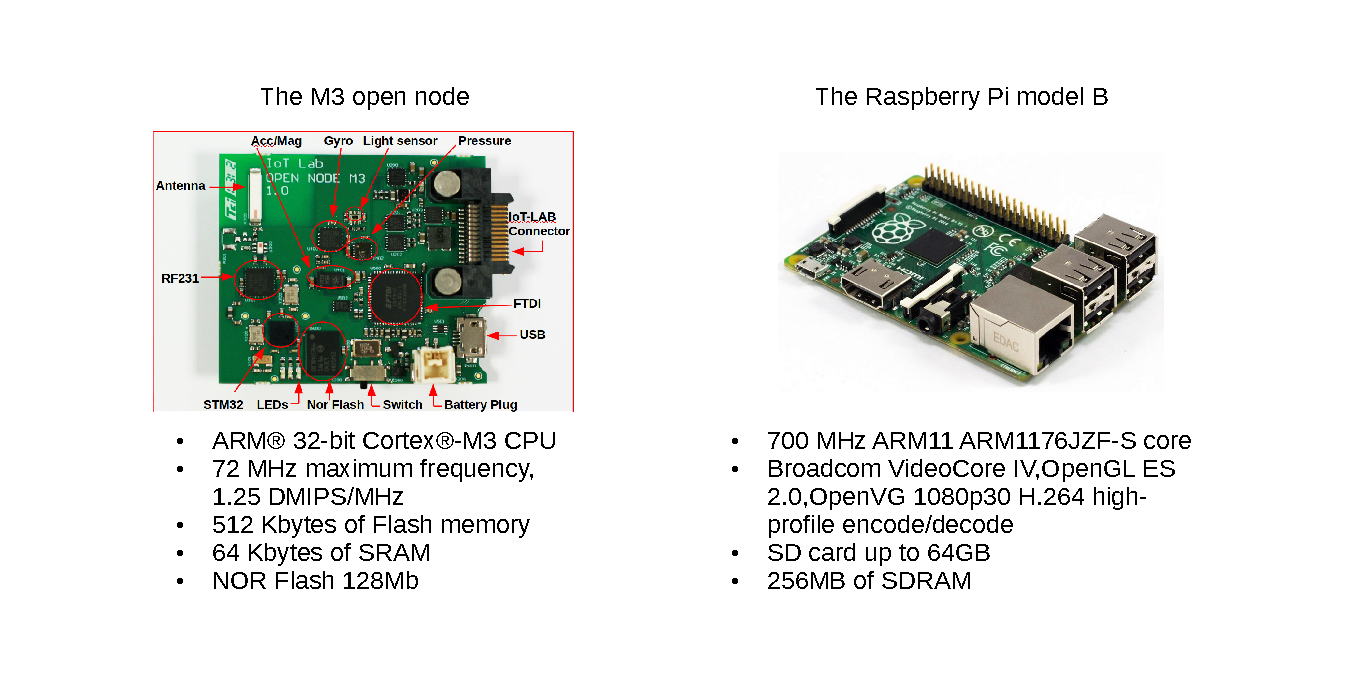
\includegraphics[width=1\columnwidth]{chapters/background.images/BoardsComparison.pdf}
	\caption{Constrained vs. non-constrained device}
	\label{fig:BoardsComparison}
\end{figure}

Figure \ref{fig:BoardsComparison} shows a resource comparison between this two kind of objects.
We can appreciate the big difference between them, as much in memory as in processing speed.
While the price and the resources of SoC systems is very attractive, power consumption still a main drawback.
Such kind of devices wouldn't last a day running in batteries, since the big amount of memory and the high speed processor are very power consuming.

The very low-cost of MCU based objects, coupled with their very low-power capabilities, make them very easy to produce and could be spread in most of physical environments, such as forests, streets, buildings and homes, since it is possible to make them run in batteries.
We can call this objects \textit{\textbf{smart objects}}.

In this thesis, I will put emphasis on MCU based smart objects, since most of the scientific challenges come with the constrained resources in memory and energy of such devices.
\begin{figure}[htb]
	\centering
	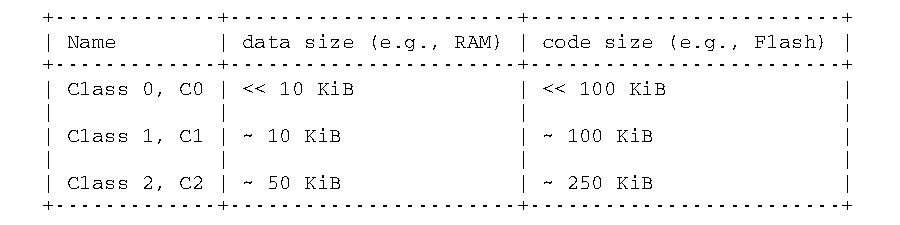
\includegraphics[width=1\columnwidth]{chapters/background.images/DeviceClass.pdf}
	\caption{Classes of constrained devices}
	\label{fig:DeviceClass}
\end{figure}
The working group light-weight implementation guidance (lwig) from the Internet Engineering Task Force (IETF) provides the very useful RFC7228\cite{rfc7228}, which separates constrained devices into classes, as depicted in figure \ref{fig:DeviceClass}.

Objects such as the M3 open node, are considered the upper limit of a constrained device, being of class 2, and are used in this thesis as the main platform for experimentations.

\subsection{The very constrained nature of MCU based smart objects}
Web technologies are nowadays well investigated and offer many tools for fast development and maintenance, however, they rely in modern equipment: fast microprocessors with many cores, tens of gigabytes in RAM and several terabytes in hard disks.
While computers, mobile phones, and similar devices grow constantly in computing capacities, for microcontrollers the evolution is much less evident.
This avoids the use of most of already developed technologies, since the differences between this two kind of devices is enormous.

One of the main reasons for this, is the cost of MCUs.
In order to maintain a very low price for this devices, the size of them should be kept small.
Since SRAM (the volatile memory type used in MCUs) takes a lot of space in the chip, it is not possible to add more without increasing the cost of the chip, which is not wanted in a very competitive market as MCUs is.
In addition, the fabrication process of MCUs differs in many ways in comparison to SRAM construction.
Thus, for semiconductor foundries a complex device fabrication leads to an increased cost.
Finally, as we stated in section \ref{sec:IoTInfra}, in the IoT flexibility in the placement of IoT devices is a major concern.
SRAM being very energy consuming, it wouldn't be possible to power large SRAM devices using batteries.
Therefore, to summarize, the construction of MCUs with huge quantities of memory is not economically viable, as well as the energy performance would be decreased.

\subsection{Communication between smart objects}
Several communication protocols are used in the classical Internet.
Most of them are based on Ethernet\cite{ieee802.3}, in which a standard cable is needed for each participant in the network.
A wireless Ethernet protocol was also standardized, as known as IEEE 802.11\cite{ieee802.11}, providing the same features without the need of cables.
Other ways to reach the current Internet also exists, such as optical fiber, satellite and different radio standards, just to name a few.

Since the IoT aims to be ubiquitous, communication using cables would complicate the physical installation of such objects.
The main advantage of MCU based objects is their very low power consumption.
Thus, a very low power communication interface would allow this objects to be powered using batteries.
Therefore, wireless communication protocols seem to be the best choice.
However, communication interfaces implementing standards i.e. IEEE 802.11, were not built having low power features in mind, making them too inefficient if batteries are used as power source.
Several wireless devices manufacturers and research institutes worked together to create new energy-aware protocols to provide wireless communication for smart objects.
One of the standards that came from these efforts was the IEEE 802.15.4\cite{ieee802.15.4}.
It was created specifically for low-power transceivers, allowing communication ranges near to 802.11, but offering a very low bandwidth.
This limitation avoid the exchange of large data packets, which also limits the protocols that can be managed by the interface, before having considerable fragmentation.

\begin{figure}[htb]
	\centering
	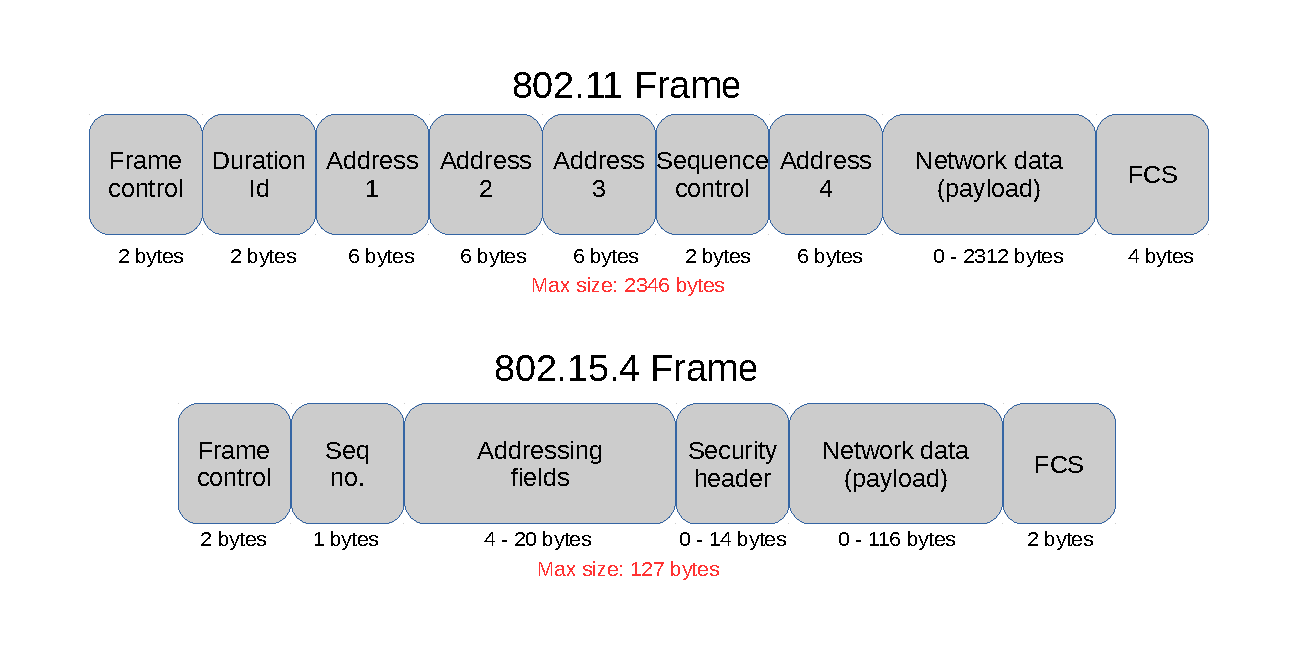
\includegraphics[width=1\columnwidth]{chapters/background.images/FramesComparison.pdf}
	\caption{Comparison in frame size between 802.11 and 802.15.4}
	\label{fig:FramesComparison}
\end{figure}

The memory constraints present in MCUs avoid the use of classical approaches to develop software for web based applications, often written in high level programming languages.
These approaches make use of common Internet protocol's implementations, which are not aware of this low resources.
Thus, a new way to provide Internet functionalities must be developed.

In 2003, Adam Dunkels developed a very lightweight TCP/IP protocol stack, uIP\cite{dunkels03full}, for 8-bit microcontrollers, enabling smart objects to communicate using a standard Internet protocol.
With this contribution, several services could be developed to create a first IoT infrastructure.
However, most of the services provided in classical Internet does not use a simple way to communicate, such as TCP/IP.
Therefore, a more complete framework for web services development should be created, to establish a more transparent and easy to use approach for resource constrained devices.

\subsection{6loWPAN, or how to give an IP address to any object}
With the arrival of the IPv6 standard\cite{rfc2460}, which enabled a wider range of IP addresses than the previous IPv4, the possibility to assign an address to each smart object became a reality.
This arise new challenges in the implementation for this new network protocol in smart objects, since the RFC2460 specification was intended for high resources machines.

Montenegro et al. proposed a new specification\cite{rfc4944} for constrained resources devices in order to communicate using IPv6 addresses.
This specification, called 6loWPAN (IPv6 for low-power Wireless Personal Area Networks) was successfully implemented\cite{durvy08making} and was able to provide interoperability with IPv6 ready devices, as it fulfilled all the requirements to have an IPv6 label\footnote{https://www.ipv6ready.org/}.
The main feature of the loWPAN adaptation layer is the compression of the IPv6 header, along with fragmentation and mesh addressing features.

\begin{figure}[htb]
	\centering
	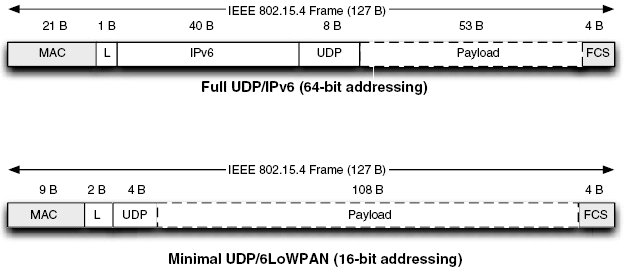
\includegraphics[width=1\columnwidth]{chapters/background.images/6lowpanvsipv6.jpg}
	\caption{IPv6 vs. 6loWPAN \cite{shelby2010embedded}}
	\label{fig:IPv6vs6loWPAN}
\end{figure}

A size comparison is done in figure \ref{fig:IPv6vs6loWPAN}.
We can appreciate that the header compression done by 6loWPAN reduces considerably its size, which is very important, given the size of IEEE 802.15.4 frames.

\begin{figure}[htb]
	\centering
	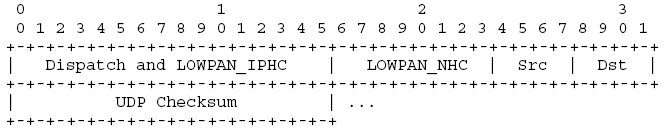
\includegraphics[width=1\columnwidth]{chapters/background.images/6lowpanDetails.jpg}
	\caption{6loWPAN header}
	\label{fig:6loWPANmin}
\end{figure}

In an ideal case, 6loWPAN headers can be as small as 6 bytes, shown in figure \ref{fig:6loWPANmin}.
This represents the "L" field in the frame.
\begin{figure}[htb]
	\centering
	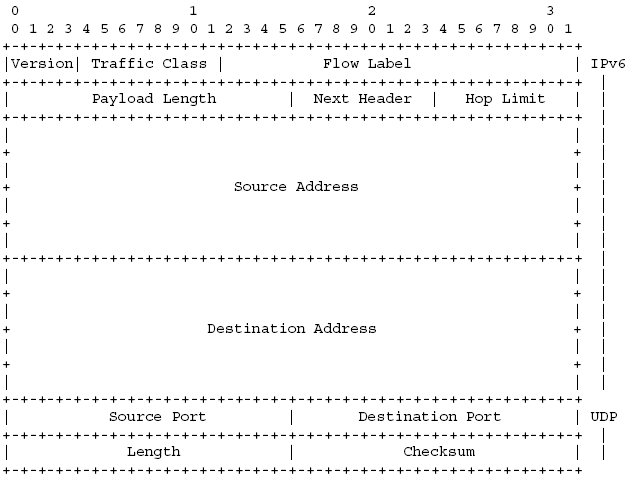
\includegraphics[width=1\columnwidth]{chapters/background.images/ipv6Details.jpg}
	\caption{IPv6 header}
	\label{fig:IPv6Header}
\end{figure}
As a comparison, the IPv6 header shown in figure \ref{fig:IPv6Header} would left only 72 bytes for payload, in the worse case.

Thanks to 6loWPAN compression, we have a first real \textit{"Internet of Things"} where every smart object can be reached from anywhere on Internet.
This enable the development of web services, since the objects themselves can already be part of a network where they can offer their embedded services, hosted in their small amount of memory.
A new way to represent this services is then required, that could meet the current web services specifications and approaches.

\subsection{An application layer for smart objects}
In the classical Internet, web services are very often represented using the HTTP application protocol\cite{rfc2616}, in an architectural style called REST, defined by Fielding and Taylor\cite{Fielding02REST}.
REST services are very useful in the web, since they have a very easy way to operate using simple verbs: GET, POST, PUT, DELETE, just to name the common ones.
This representation could be also useful for smart objects, allowing the user, or other smart objects, to access its services in a standard way, providing interoperability with a good abstraction level.

While an implementation of HTTP is conceivable for smart objects, the huge amount of memory in both RAM and ROM turn it too heavy and inefficient to run on constrained, battery-powered devices\cite{Shelby10EWS}.
To solve this problem, Shelby et al. standardized the "HTTP for resource constrained devices"\cite{rfc7252}, called CoAP (Constrained Application Protocol).
This new application protocol is able to manage the methods described above, fulfilling the requirements for a RESTful API.
\begin{figure}[htb]
	\centering
	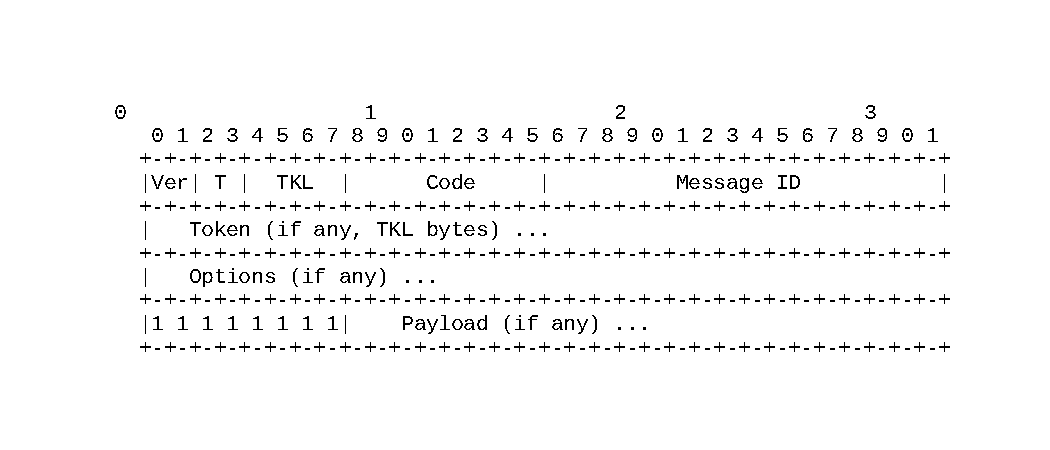
\includegraphics[width=1\columnwidth]{chapters/background.images/CoAPMessageFormat.pdf}
	\caption{CoAP Message format}
	\label{fig:CoAPMessageFormat}
\end{figure}
Figure \ref{fig:CoAPMessageFormat} shows a typical CoAP message, in which we can see that only 13 bytes are needed to format this message, allowing the rest of the frame for payload.

The services provided by the smart objects can be represented in a HTTP like form, i.e. \texttt{/sensors/temperature} for a temperature resource. If we use the CoAP command GET for this resource, we should have a response similar to "22.5", as an example of resource representation.
The PUT and POST commands are used to change the state of the actuators that can be present in a smart object.
For instance, if we want to change the state of a LED, we access the resource \texttt{/leds} with a query \texttt{?color=red} for a red LED, and a payload \texttt{mode=on} in order to turn it on.
This API facilitates the exchange of information between other smart objects, as known as "Machine to Machine (M2M)" communication.

CoAP was also developed having in mind the interoperability issue that comes when we need to communicate with other machines, which don't use CoAP as application protocol, providing an easy way to translate the messages to HTTP.

\section{Overview of the protocol stacks}
Having described a smart object capacities and capabilities, we can now make a layered comparison between the classical Internet and the IoT protocols stacks, built from the protocols already mentioned above.

\begin{figure}[htb]
	\centering
	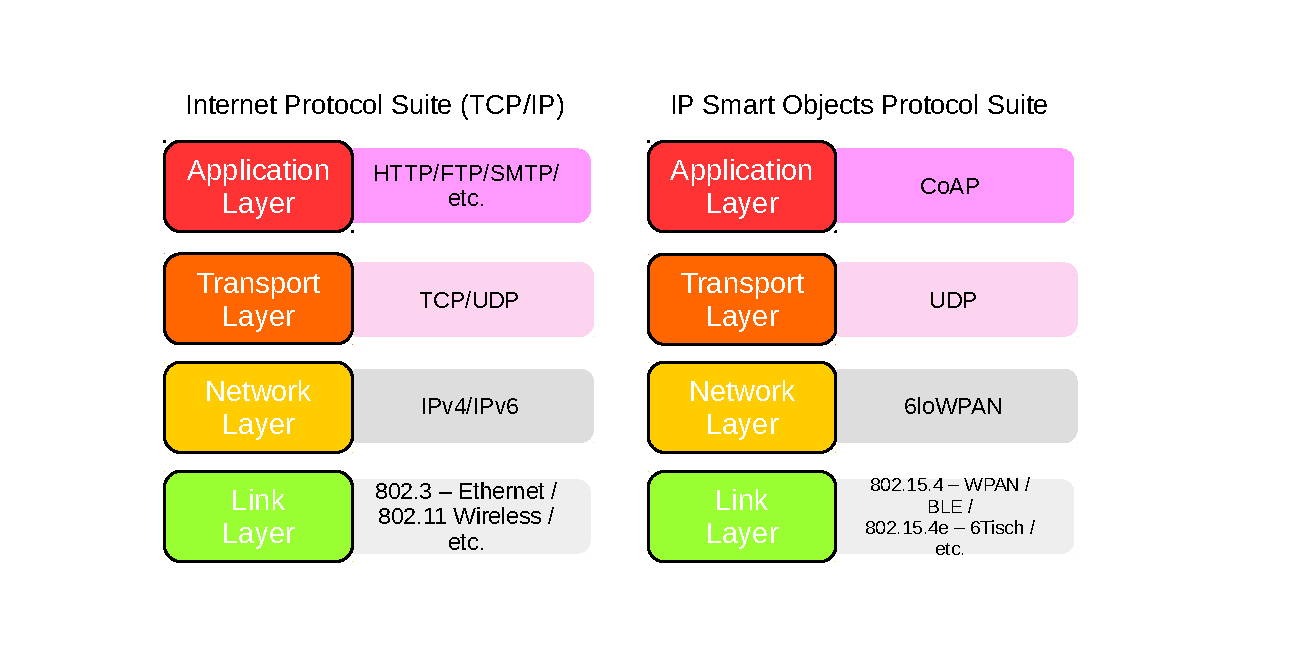
\includegraphics[width=1\columnwidth]{chapters/background.images/Layers.pdf}
	\caption{Comparison between Internet protocols stacks}
	\label{fig:IPLayers}
\end{figure}

In figure \ref{fig:IPLayers} we can appreciate a layered representation of both stacks, the classical Internet and the IoT.
This view allows a general understanding of some of the protocols that can enable the Internet of Things infrastructure.
Both stacks are able to communicate between them, allowing users and developers to mix different types of smart objects, as well as other types of devices that can participate in the same network, such as PCs, servers and so on.

In section \ref{sec:BAScenario} the representation of the building services shows that, after an IP layer, the data access is done through cloud services, which provide web APIs for further use by any web application.
The presented protocol stack is the proposed way to directly communicate with this cloud services, using a standard way to ease the development, test, and continuous integration of web services.



%\subsection{Other IP stacks for smart objects}
%Other protocol stacks provide similar behavior than the mentioned above.
%Several use privative protocols that limit the interoperability, which is very important when the connected smart objects to the IoT can reach several billions\footnote{http://www.cisco.com/web/solutions/trends/iot/portfolio.html}.
%In the home and building automation domain, we can find for instance: BacNET/IP, KNX/IP, LonWorks/IP, and so on.
%The wired communication bus used in these technologies, limits the possibility of spreading the objects in all environments, as described in section \ref{sec:IoTInfra}.
%Although wireless specifications can exist for some of them\footnote{http://www.weinzierl.de/download/products/730/KNX\_over\_IP\_EN.pdf}, the IP connectivity is only achieved using specific gateways that can encapsulate/de-capsulate the basic protocol for IP use.
%Thus, there is no a transparent nor easy way to communicate with this objects.
%This main drawback makes not viable the use of these protocols in an IoT infrastructure.

\section{All-in-one: IoT operating systems}
In the classical Internet, several operating systems (OS) are used to take advantage of the services provided on the web.
An operating system provides all the necessary software to manipulate web content, based on user needs.
We can find, for instance, web browsers, mail clients, file managers, audio streamers, and so on, which use several Internet protocols already provided by the OS.

A similar need comes with the IoT.
However, web content in the IoT is not intended to be used directly by humans, but for other machines that gather such content and process it to offer new services.
Therefore, an operating system for the IoT should integrate all the necessary tools to provide a full communication stack, as well as a friendly environment to ease the development of applications.
In this section, some operating systems that provides such functionalities are described.

\subsection{Contiki}
Developed at the beginning for Wireless Sensor Networks (WSN) management, the Contiki OS\cite{dunkels2004contiki} provides a full network stack composed of several communication protocols, from the network to the application layers.
Built as a monolithic event-driven kernel, as well as modular, Contiki offers a standard way to develop applications, following a structured architecture of \textit{processes}.

Written in C, this OS and their applications can be compiled for several infrastructures, as Contiki provides enough abstractions to be platform independent.
The most common MCU architectures using this OS are msp430, AVR, ARM, among others.
The amount of memory needed in a 16-bit microprocessor (i.e. msp430) is about 2KB of RAM and 40KB of ROM.

\subsubsection{IoT protocol stack}
\begin{figure}[htb]
	\centering
	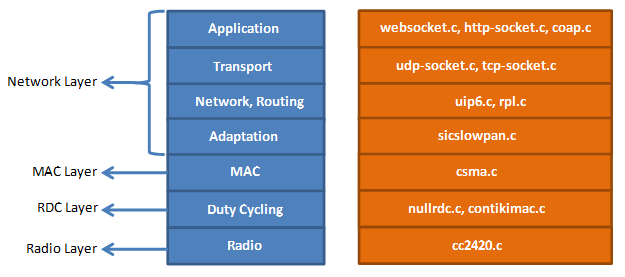
\includegraphics[width=1\columnwidth]{chapters/background.images/Contikinetstack.png}
	\caption{Contiki general network stack on the left (in blue) \& corresponding  netstack source codes on the right (in orange)}\footnote{Source files according to \url{https://github.com/contiki-os/contiki/tree/release-3-0}}
	\label{fig:ContikiNetStack}
\end{figure}
After several years of development, Contiki became an IoT OS by adding an IP Smart Object stack, which is described in figure \ref{fig:ContikiNetStack}.
Moreover, Contiki provides the following additional features:
\begin{itemize}
	\item Duty Cycling. ContikiMAC\cite{dunkels2011contikimac} is a radio duty cycling protocol that uses periodical wake-ups to listen for packet transmissions from neighbors.
	Since radio communication is the most energy consuming task, this feature reduces considerably the power consumption.
	\item MAC. An implementation of CSMA/CA that avoids collisions before sending a radio packet.
	\item Adaptation. SICSloWPAN is the Contiki implementation of the 6loWPAN RFC\cite{rfc4944}.
	\item Routing. ContikiRPL\cite{tsiftes2010contikirpl} implements the RPL\cite{rfc6550} protocol, which is an IPv6 Routing Protocol for Low-Power and Lossy Networks. RPL organizes a	topology as a Directed Acyclic Graph (DAG) that is partitioned into one or more Destination Oriented DAGs (DODAGs), one DODAG per sink.
\end{itemize}

\subsubsection{Main OS features}
In addition to a very complete IP stack, Contiki integrates other useful features:

\begin{itemize}
	\item Multitasking kernel.
	\item Preemptive multi-threading.
	\item Proto-threads\cite{dunkels2006protothreads}.
	\item The RIME communication stack\cite{dunkels2007rime}.
	\item The Coffee file system\cite{tsiftes09enabling}.
	\item A dynamic loader of new modules\cite{dunkels06runtime}.
\end{itemize}

The multitasking kernel, in addition to proto-threads, are the core of this OS.
This features makes the organization of applications very simple, since adding a new process creates automatically a new proto-thread, which is accessible through event-passing.
A list of events is also available, giving to the user the possibility to create custom events, in addition to the existing ones.
Depending on the needs, events are dispatched following a First In First Out (FIFO) approach when asynchronous events are used, and direct passing for synchronous events.
This is the main way to communicate between process, allowing to pass memory pointers between each poll.

\subsubsection{The Coffee file system}
In a classical OS a file system is a mandatory feature.
Indeed, storing files and programs is one of the main functionalities that an OS can provide.
This is needed as much as for program execution, as for data logging and configurations storage.
While constrained smart objects have often a persistent data storage, such as flash memory or EEPROM, a versatile and easy to use approach to access the saved data is always useful.
The coffee file system, using default settings, needs only 5KB of ROM and 0.5KB of RAM at runtime.
This is a decent amount of memory regarding the benefits that a file system brings to an OS.
It uses typical methods to access files, such as \texttt{cfs\_open(), cfs\_close(), cfs\_read() and cfs\_write()}, which take as parameters the filename as a string and its options for opening (\texttt{CFS\_READ, CFS\_WRITE or CFS\_APPEND}).
Moreover, the design was intended for flash memory, which has a limited write/erase cycles.
Coffee leverage a garbage collection system that erase memory only when there is no more available pages to write, which reduces considerably the write/erase cycles compared to direct flash access.

This file system enables very important features needed for the proposed IoT infrastructure.
Logging data locally for further use can be very useful, but storing configurations and data about network behavior is even more.
Furthermore, easy storage and access to program data in a binary file form can enable firmware replacement, either fully or partially.
This is achieved by Contiki through the dynamic loader, which is described below.

\subsubsection{The dynamic loader}
One of the most appreciable features in an OS is its possibility to update existing capabilities, or adding new ones.
Contiki provides a dynamic linker at runtime, which is able to load binary code using the standard ELF format\cite{tis1995tool}.
Leveraging the abstractions already done by the Coffee File System (CFS), this dynamic loader does not need to know whether the code is located in RAM or ROM, since the CFS manages this low-level details.
Since Contiki was designed to be modular, only the core contains important program code.
This means that any other module can be replaceable by a new one (i.e. network stack, sensing applications, etc.), thus allowing correct bugs.

\begin{figure}[htb]
	\centering
	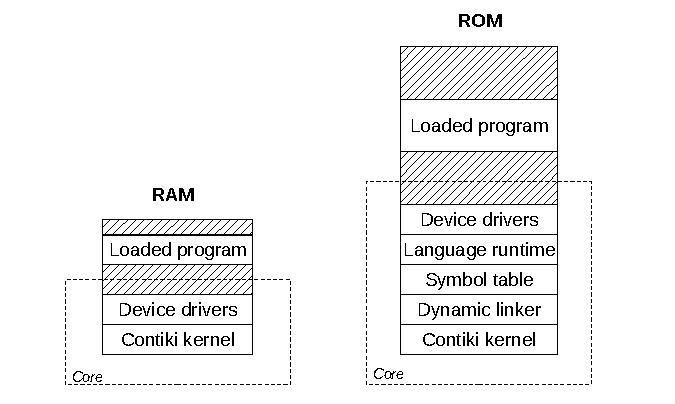
\includegraphics[width=1\columnwidth]{chapters/background.images/ContikiModules.pdf}
	\caption{Partitioning in Contiki: The core and loadable programs in RAM and ROM\cite{dunkels06runtime}}
	\label{fig:ContikiModules}
\end{figure}

Figure \ref{fig:ContikiModules} shows the minimal modules embedded in Contiki, leaving free space for new ones.


\subsection{RIOT}
RIOT is an IoT operating system\cite{baccelli2013riot}, with a microkernel architecture.
It supports a full IP stack for smart objects, offering interoperability with other OS like Contiki.
It's very low memory footprint make it ideal for IoT, since it can be compiled for several architectures, from 8-bit to modern 32-bit microcontrollers.

It's main features can be described as follows:

\begin{itemize}
	\item Microkernel (for robustness)
	\item Modular structure to deal with varying requirements
	\item Tickless scheduler
	\item Deterministic kernel behaviour
	\item Low latency interrupt handling
	\item POSIX like API
	\item Native port for testing and debugging
\end{itemize}

As we can see, RIOT has a very different architecture than Contiki, its close competitor.
However, the IP stack is very similar.
It uses the same protocols as Contiki, but the implementations follow different approaches.

\begin{figure}[htb]
	\centering
	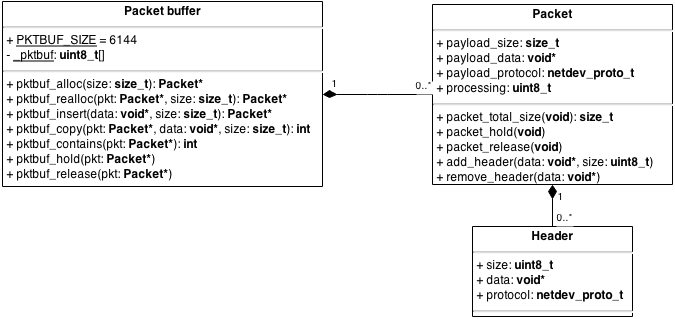
\includegraphics[width=1\columnwidth]{chapters/background.images/pktbuf-uml-class.png}
	\caption{RIOT packet UML classes}
	\label{fig:RIOTpktBuf}
\end{figure}

It uses a generic packet buffer which can send packets either for IPv6 or IPv4.
The model of this packets is shown in figure \ref{fig:RIOTpktBuf}.
Up to beginning 2014, RIOT had a network stack more or less complete, with most of the implementations already working.
Given the IoT infrastructure proposed in section \ref{sec:IoTInfra}, RIOT fulfill almost all requirements, with the exception of RPL and CoAP.

\begin{figure}[htb]
	\centering
	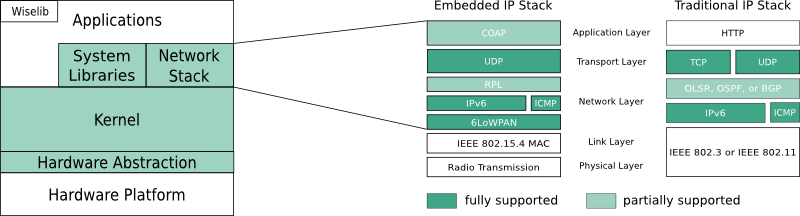
\includegraphics[width=1\columnwidth]{chapters/background.images/RIOTIPStack.png}
	\caption{RIOT IP stack}
	\label{fig:RIOTIPStack}
\end{figure}

Figure \ref{fig:RIOTIPStack} show the comparison between protocols and the support offered by this OS. 

\begin{table}[htb]
	\centering
	\caption{OS comparison}
	\label{tab:OSComparison}
	\begin{tabular}{|c|cccccccc}
		\hline
		\textbf{OS} & 
		\multicolumn{1}{p{0.8cm}|}{\textbf{Min} \newline \textbf{RAM}} &
		\multicolumn{1}{p{0.8cm}|}{\textbf{Min} \newline \textbf{ROM}} &
		\multicolumn{1}{p{1.3cm}|}{\textbf{C} \newline \textbf{Support}} &
		\multicolumn{1}{p{1.3cm}|}{\textbf{C++} \newline \textbf{Support}} &
		\multicolumn{1}{p{1.6cm}|}{\textbf{Multi} \newline \textbf{Threading}} &
		\multicolumn{1}{p{1cm}|}{\textbf{MCU} \newline \textbf{w/o} \newline \textbf{MMU}} &
		\multicolumn{1}{c|}{\textbf{Modularity}} &
		\multicolumn{1}{c|}{\textbf{Real-time}} \\ \hline
		\textit{Contiki} & \textless 2KB & \textless 30KB &$\bullet$ & \textbf{x}       & $\bullet$     & \checkmark     &$\bullet$ &    $\bullet$ \\ \cline{1-1}
		\textit{TinyOS}  & \textless 1KB & \textless 4KB  &\textbf{x}& \textbf{x}       & $\bullet$     & \checkmark     &\textbf{x}&   \textbf{x}\\ \cline{1-1}
		\textit{Linux}   & $\mathtt{\sim}$1MB &$\mathtt{\sim}$1MB&\checkmark & \checkmark       &  \checkmark   & \textbf{x} &$\bullet$   &$\bullet$    \\ \cline{1-1}
		\textit{RIOT} & $\mathtt{\sim}$1.5KB & $\mathtt{\sim}$1.5KB & \checkmark    & \checkmark       & \checkmark & \checkmark & \checkmark & \checkmark  \\ \cline{1-1}
	\end{tabular}
\end{table}

In this table, \textbf{x} represent no support, $\bullet$ partial support and $\checkmark$ fully support.

In table \ref{tab:OSComparison} a comparison between OS is made.
It shows that RIOT offers several features that other OS cannot, having remarkable advantages such as size and programming options.

Two main drawbacks were found in this OS:
\begin{enumerate}
	\item The lack of a flexible and easy to use approach to store data in persistent memory.
	\item A method to replace or add new features.
\end{enumerate}

Even if the very attractive programming model (C++ availability) is useful to implement self-adaptation and reconfiguration approaches, the lack of this two vital functionalities in our IoT infrastructure is a big inconvenient, our goals being to provide an easy way to adapt it and to reconfigure it.
Given that configuration files must be stored in external flash memory, and a dynamic loader which uses binary files with new applications, this OS was discarded for the use on this thesis.

\section{Other embedded OS}


\subsection{TinyOS}
bla

\section{Enabling adaptation and reconfiguration in the IoT}
One of the main goals of the proposed IoT infrastructure is to offer their capabilities through web services.
Once this goal achieved by related research, our goal in this thesis is to leverage this new web technologies to provide adaptation and reconfiguration capabilities.
Previous works using approaches typical of Model Driven Engineering (MDE), have obtained good results adding self-adaptation and reconfiguration mechanisms to distributed systems.

One of this approaches is Models@runtime\cite{morin2009mar}.
Under this perspective, we aim to represent the IoT infrastructure described in this chapter, in the form of a model at runtime.
We leverage its main properties to provide an easy way to manage reconfigurations, new software deployment and updates.
Further discussion about this topic is conducted in the next chapter.

